% Chapter 1
\chapter{Background: statistical modeling of calcium imaging data}
\chaptermark{Background}


\section{Overview of calcium imaging data} 

Calcium ions generate intracellular signals that control key functions in all types of neurons.
At rest, most neurons have an intracellular calcium concentration of about 100 nm; however, during electrical activity, the concentration can rise transiently up to levels around 1000 nm~\citep{berridge2000}. 
The development of techniques that enable the visualization and quantitative estimation of the intracellular calcium signals have thus greatly enhanced the investigation of neuronal functioning.
The development of calcium imaging techniques involved two parallel processes: the development of calcium indicators, which are fluorescent molecules that react when binding to the calcium ions, and the implementation of the appropriate imaging instrumentation, in particular, the introduction of two-photon microscopy~\citep{denk1990}.
In recent years, the innovation achieved in these two fields has allowed for real-time observation of biological processes at the single-cell level simultaneously for large groups of neurons~\citep{grienberger2012}. 

The output of two-photon calcium imaging is a movie of time-varying fluorescence intensities, and a first complex pre-processing phase deals with the identification of the spatial location of each neuron in the optical field and source extraction~\citep{mukamel2009,dombeck2010}. The resulting processed data consist of a fluorescent calcium trace for each observable neuron in the targeted area which, however, is only a proxy of the underlying neuronal activity.
Hence further analyses are needed to deconvolve the fluorescence trace to extract the spike train (i.e. the series of recorded firing times), and to try to explain how these firing events are linked with the experiment that generated that particular pattern of activity.

\subsection{Deconvolution methods}
\label{ch1_sec:deconvolution_methods}

There is currently a rich literature of methods addressing the issue of deconvolving the raw fluorescent trace to extract the spike train. A successful approach is to assume a biophysical model to relate the spiking activity to the calcium dynamics, and to the observed fluorescence. \citet{vogelstein2010} proposed a simple but effective model that has later been adopted by several authors~\citep{pnevmatikakis2016, friedrich2016, friedrich2017, jewell2018, jewell2019}. The model considers the observed fluorescence as a linear (and noisy) function of the intracellular calcium concentration; the calcium dynamics is then modeled using an autoregressive process with jumps in correspondence of the neuron's firing events.
Denoting with $y_t$ the observed fluorescence trace of a neuron and with $\Ca_t$ the underlying calcium concentration, for time $t=1,\dots,T$, the model can be written as
\begin{equation}
\begin{gathered}
y_t = b + \Ca_t + \epsilon_t,\quad \epsilon_t \sim \N(0,\sigma^2),  \\
\Ca_t = \gamma\, \Ca_{t-1} + A_t + w_t, \quad w_t \sim \N(0, \tau^2),
\end{gathered}
\label{ch1_eq:armodel}
\end{equation}
where $b$ models the baseline level of the observed trace and $\epsilon_t$ is a Gaussian measurement error. In the absence of neuronal activity, the true calcium concentration $\Ca_t$ is considered to be centered around zero. The parameter $A_t$ captures the neuronal activity: in the absence of a spike ($A_t = 0$), the calcium level follows a AR(1) process controlled by the parameter $\gamma$; when a spike occurs, the concentration increases instantaneously of a value $A_t > 0$.
A challenge remains estimating the neuronal activity $A_t$ in a precise and computationally efficient way.

\citet{vogelstein2010} assumed that all spikes have a fixed amplitude, and interpreted the parameter $A_t$ as the \textit{number} of spikes at time $t$. Following this definition, they placed a Poisson prior distribution on $A_t$; however, the maximum a posteriori estimation of the spike train using a Poisson distribution is computationally intractable. Hence they searched an approximate solution by replacing the Poisson distribution with an exponential distribution of the same mean. This leads to some loss of interpretation of the parameters $A_t$, as now they are no longer integer values but rather non-negative real numbers, but turns the problem into a convex optimization, which can be solved efficiently.
Adopting this approach leads to solving a non-negative lasso problem for estimating the calcium concentration, where the $L_1$ penalty enforces sparsity of the neural activity.
Efficient algorithms to obtain a solution of this problem have also been proposed by \citet{pnevmatikakis2016}, \citet{friedrich2016}, and \citet{friedrich2017}.

A different perspective is instead proposed by~\citet{jewell2018} and~\citet{jewell2019}: rather than interpreting $A_t$ in model~(\ref{ch1_eq:armodel}) as the number of spikes at the $t$-th timestep, they interpreted its sign as an indicator for whether or not \textit{at least one} spike occurred, that is, $A_t = 0$ indicates no spikes at time $t$, and $A_t>0$ indicates the occurrence of at least one spike. The model so formulated includes an indicator variable, which corresponds to using an $L_0$ penalization and which makes the optimization problem highly non-convex. 
In their work, \citet{jewell2018} and~\citet{jewell2019} developed fast algorithms to compute the spike trains under these assumptions.
\citet{jewell2018} asserted that the solutions discussed by \citet{vogelstein2010}, \citet{friedrich2016}, and \citet{friedrich2017} can actually be seen as convex relaxations of this optimization problem, to overcome the computational intractability of the $L_0$ penalization. 

Finally,~\citet{pnevmatikakis2013} proposed a fully Bayesian approach. Although less computationally efficient than optimization methods, it allows to obtain a posterior distribution of all model parameters instead of just a point estimate, hence improving uncertainty quantification.
Differently from previous models, they defined the parameter $A_t$ as the \textit{amplitude} of a spike at time $t$, taking values in the non-negative real numbers.
They formulated the presence/absence of a spike and its amplitude by using the product of a Bernoulli random variable (taking value 0 if there is no spike at time $t$, and 1 otherwise) with a half-Gaussian random variable (modeling the positive amplitudes). However, they did not explicitly assume sparsity of the spikes.


\subsection{Spike train data analysis}
\label{ch1_sec:spike_train_analysis}
Standard methods to analyze calcium imaging data rely on a two-step approach: in a first phase, some deconvolution method such as those just described is applied to identify the spikes, then, a different method is used on the deconvolved output to analyze it and, possibly, to relate it with some covariates.
However, while there is a rich literature on deconvolution methods, there is still little research on methods that try to derive inferential results from their output.

Concerning encoding models, i.e. models that try to understand how the brain encodes external variables into spike train, \citet{paninski2007} focused on the use of generalized linear models (GLMs). GLMs allow spike trains to be regressed against a potentially large number of covariates such as behavioral parameters, experimental conditions and other relevant factors.
Moreover, regression models provide simple and interpretable results of the effect of each covariate on the neuronal response.
In particular, \citet{paninski2007} highlighted the importance of regularization methods and inclusion of prior knowledge to improve estimation of the model parameters, as in many cases the number of covariates is potentially very large, leading to noisy results and a loss in interpretability.

A different approach has been proposed by \citet{wei2019}: instead of focusing the relationship between the experimental conditions and some summary statistic of the resulting spike train, they studied the distribution of the deconvolved output. In particular, this allows to analyze quantities such as the spike probability and the spikes' amplitudes. They proposed a mixture model, with a Dirac mass at zero, representing the absence of neuronal response, and a translated Gamma distribution to model the positive amplitudes.

\section{Data sets} 
Una frase introduttiva? Parlo dei dati dell'Allen Brain Observatory e poi ci sarebbe da mettere i nuovi dati se riesco a fare qualcosa del progetto 3...

\subsection{Allen Brain Observatory data}
\label{ch1_sec:allen_brain_data}
The Allen Brain Observatory~\citep{allen} is a large public data repository for investigating how sensory stimulation is represented by neural activity in the mouse visual cortex in both single cells and populations.
The project aims to provide a standardized and systematic survey to measure and analyze visual responses from neurons across cortical areas and layers, utilizing transgenic Cre lines to drive expression of genetically encoded fluorescent calcium indicators, and measured by \textit{in vivo} two-photon calcium imaging.

The study is an extended survey of physiological activity in the mouse visual cortex in response to a range of visual stimuli~\citep{allen_stimulus}. Each mouse was placed in front of a screen where different types of visual stimuli were shown, while the mouse’s neuronal activity was recorded. The stimuli vary from simple synthetic images such as locally sparse noise or static gratings, to complex natural scenes and movies.
The goal of the study is to investigate how neurons at different depths and in different areas of the visual cortex respond to stimuli of varying complexity, to understand their functional properties. Specifically, each neuron in the visual cortex can be characterized by their \textit{receptive field}, i.e. the features of the visual stimulus that trigger the signaling of that neuron. 
An important finding from mammalian is that higher visual areas tend to respond to more complex stimuli relative to lower areas. These differences indicate that the different neurons and visual areas have distinct functional properties.
Hence, it is of critical interest to devise methods that allow inferring how the neuronal response varies under the different types of visual stimuli. %We expect that the neuronal activity will vary across all the experimental settings, and that some variations in its intensity will be observed based on the specific visual stimulus.
As an example, Figure \ref{ch1_fig:trace_neurons} shows the calcium traces of two neurons recorded during two different experiment sessions from the Allen Brain Observatory study.
Each experiment comprises three types of visual stimuli, and has a duration of approximately one hour.
These plots highlight that the neuronal response is highly variable, both across experimental conditions and between neurons.

\begin{figure}
	\centering
	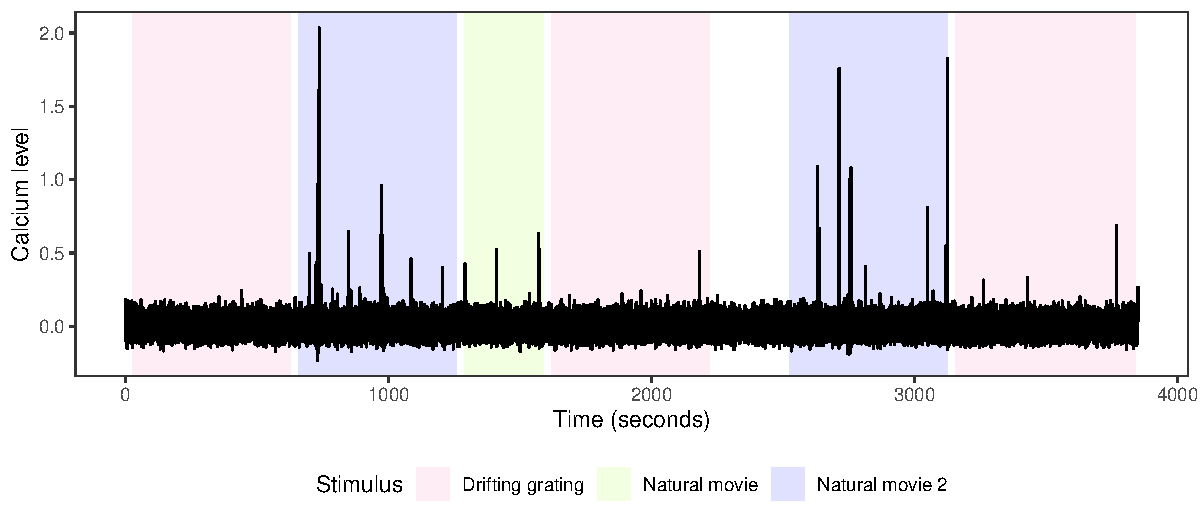
\includegraphics[width=.9\textwidth]{ch1_neuron2_trace}
	\centering
	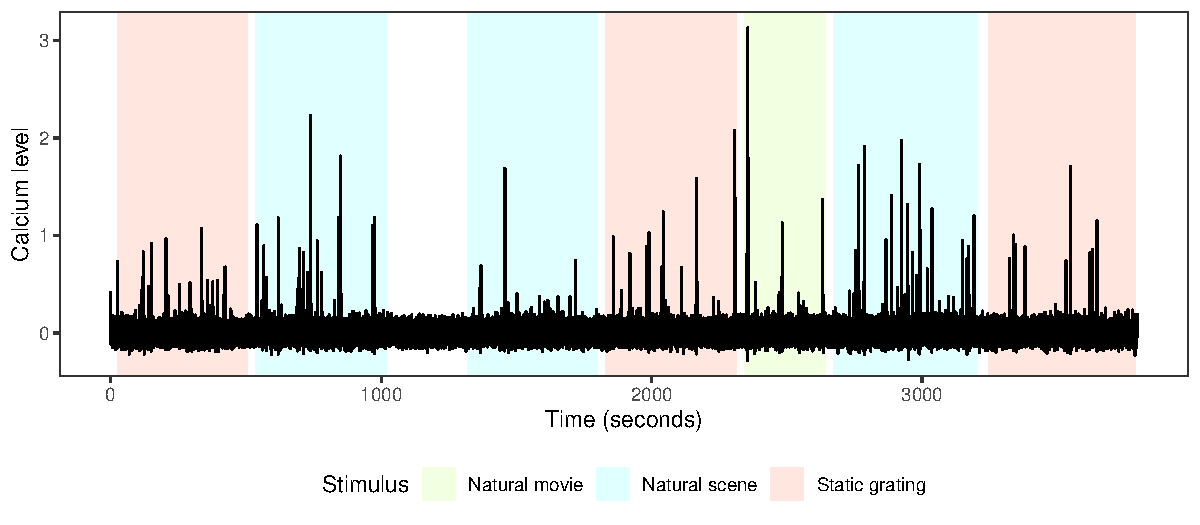
\includegraphics[width=.9\textwidth]{ch1_neuron1_trace}
	\caption[Allen Brain Observatory data: calcium traces of two neurons located in the primary visual area during Session A and Session B of the experiment. ]{Allen Brain Observatory data: calcium traces (black line) of two neurons located in the primary visual area during Session A (upper plot) and Session B (bottom plot) of the experiment. The background colors denote the visual stimulus displayed at each time.}\label{ch1_fig:trace_neurons}
\end{figure}

The Allen Brain Observatory study comprises records of neuronal activity from over $60000$ cells from six visual areas (VISp, VISl, VISal, VISrl, VISam, and VISpm) and different imaging depths (ranging from 175 to 625 microns). The data were collected analyzing the brain activity of several genetically engineered mice, using different transgenic Cre lines.
The neuronal response of each mouse was recorded during three experimental sessions: specifically, each session was made up of different types of visual stimuli displayed sequentially.
Session ``A'' comprises two natural movies and a drifting gratings stimulus; session ``B'' comprises both natural movies and natural scenes, and a static gratings stimulus; finally, session ``C'' again includes two natural movies, and a locally sparse noise. Moreover, in all sessions a period of absence of stimuli was used to evaluate the baseline response during spontaneous activity.
The synthetic stimuli are used to investigate the parameters that trigger the neuronal response: the locally sparse noise displays white and black spots in different parts of the visual space, and allows to map the spatial size and shape of the receptive field. The grating stimulus is a simple pattern whose intensity varies periodically along one dimension, and is constant in the other dimension. Different spatial frequencies, temporal frequencies and orientations are considered in order to further characterize the receptive fields. A detailed description of the visual stimuli can be found in a technical report \citep{allen_stimulus}.





\subsection{Altri dati?}
Paragrafo qui.
















\sectionmark{Bayesian nonparametric models}
\section{A brief review of some Bayesian nonparametric models} 
\sectionmark{Bayesian nonparametric models}
In this section we review some statistical tools that will be employed in this thesis in the analysis of calcium imaging data. The purpose of this section is not to provide a comprehensive review, but rather to outline the theoretical framework we adopted and fix some notation.
The core topic will be the Bayesian methodology, with a focus on Bayesian nonparametric models.

\subsection{Finite mixture models}
\label{ch1_sec:finite_mix}
We start our discussion by reviewing finite mixtures. Although they are not part of the Bayesian nonparametric methodology, they provide the starting point for many models that we will review in the following. The content of this brief overview on finite mixtures is largely based on the dedicated chapter in~\citet{gelman2013}.

\subsubsection*{Definition and hierarchical representations}
Mixtures are a popular tool to model heterogeneous data, characterized by the presence of subpopulations within the overall population. In many practical problems the data are collected under different conditions -- unfortunately, it is not always possible to have information on the subpopulation to which each individual observation belongs.
Mixture models can be used in problems of this type, where the population consists of a number of latent subpopulations, and within each of them a relatively simple model can be applied.

Denote the observed data as a vector of $n$ units $\bm{y} = (y_1,\dots,y_n)$; also, assume that the $n$ observations are exchangeable, meaning that the joint probability density $p(y_1,\dots,y_n)$ is invariant to permutations of the indices. In the framework of finite mixtures, we assume that the population is made of $K\leq n$ subpopulations, with $K$ known and fixed.
We assume that within each of these groups, the distribution of $y_i$, $i=1,\dots,n$, can be modeled as $f(y_i \mid \theta_k^*)$, for $k=1,\dots,K$. Usually a common parametric family is assumed for all these component distributions, which however depend on specific parameter vectors $\theta_k^*$.
The last missing piece to construct a mixture model is the parameter describing the proportion of population from each component $k$: we denote this parameter with $\pi_k$, satisfying $\sum_{k=1}^K \pi_k = 1$. Denoting the full vectors of parameters as $\bm{\theta}^* = (\theta_1^*,\dots,\theta_K^*)$ and $\bm{\pi} = (\pi_1,\dots,\pi_K)$, the data distribution for observation $i$ can be formulated as
\begin{equation*}
p(y_i\mid \bm{\theta}^*,\bm{\pi}) = \pi_1 \, f(y_i\mid\theta_1^*) + \dots + \pi_K \, f(y_i\mid\theta_K^*).
\end{equation*}

In mixture models it is convenient to think of the component indicators as missing data, and to impute them to obtain a much simpler form of the data distribution. Hence we introduce the indicator $S_{ik}$ of component $k$ for observation $i$, with 
\begin{equation*}
S_{ik} = \begin{cases}
1 \quad \text{if $y_i$ is drawn from component $k$}\\
0 \quad \text{otherwise}.
\end{cases}
\end{equation*}
Given $\bm{\pi}$, the distribution of $\bm{S}_i = (S_{i1},\dots,S_{iK})$ is $\Mult(1;\pi_1,\dots,\pi_K)$. 
Conditionally on $\bm{S}_{i}$, the data distribution of $y_i$ is simply $p(y_i\mid \bm{S}_i,\bm{\theta}^*) = \prod_{k=1}^K f(y_i\mid\theta_k^*)^{S_{ik}}$; moreover, given $\bm{S}=(\bm{S}_1,\dots,\bm{S}_n)$, the $y_i$ are assumed to be independent.
The joint density of the observed data and the unobserved indicators, conditionally on the model parameters, can now be written as 
\begin{equation*}
p(\bm{y},\bm{S}\mid \bm{\theta}^*,\bm{\pi}) = p(\bm{y}\mid\bm{S},\bm{\theta}^*)\, p(\bm{S}\mid\bm{\pi}) = 
\prod_{i=1}^n \prod_{k=1}^K \left\{ \pi_k f(y_i\mid\theta_k^*) \right\}^{S_{ik}}.
\end{equation*}

Having defined the data distribution, we need to specify adequate prior distributions on the model parameters $\bm{\pi}$ and $\bm{\theta}^*$. The prior $G_0$ on $\bm{\theta}^*$ is usually chosen depending on the specific application and on the basis of the component distribution $f$. For the mixture proportions $\pi_k$, the conjugate and most natural prior distribution is the Dirichlet distribution, $\bm{\pi}\sim \Dir_K(\alpha_1,\dots,\alpha_K)$.

This model also admits a useful hierarchical representation. Rewriting the latent allocation variables using the cluster indicators $c_i\in\{1,\dots,K\}$, with $c_i=k$ if $y_i$ belongs to the $k$-th mixture component (i.e. $S_{ik} = 1$), the model is, for $i = 1,\dots,n$ 
\begin{equation}
\begin{gathered}
y_i \mid c_i = k, \theta^*_k \sim f(y_i\mid\theta^*_k)\\
\Pr(c_i = k \mid \pi_1,\dots,\pi_K) = \pi_k \quad \text{for } k = 1,\dots,K\\ 
\theta^*_1,\dots,\theta^*_K \sim G_0\\
\pi_1,\dots,\pi_K  \sim \Dir_K(\alpha_1,\dots,\alpha_K).
\end{gathered}
\label{ch1_eq:finitemix_h1}
\end{equation}

It is possible to rewrite Equation (\ref{ch1_eq:finitemix_h1}) in a slightly different way by thinking that each observation $y_i$ is associated with a parameter $\theta_i$, where these parameters are drawn from a discrete distribution $G$ with support on the $K$ locations $\{\theta^*_1,\dots,\theta^*_K\}$. The model then becomes, for $i=1,\dots,n$
\begin{equation}
\begin{gathered}
y_i \mid \theta_i \sim f(y_i\mid\theta_i)\\
\theta_i \mid \bm{\theta}^*,\bm{\pi} \sim G = \sum_{k=1}^K \pi_k \delta_{\theta^*_k}\\
\theta^*_1,\dots,\theta^*_K \sim G_0\\
\pi_1,\dots,\pi_K \sim \Dir_K(\alpha_1,\dots,\alpha_K).
\end{gathered}
\label{ch1_eq:finitemix_h2}
\end{equation}

\subsubsection*{Posterior inference for finite mixture models}
Posterior inference for mixture models is usually performed through Markov Chain Monte Carlo (MCMC) methods and, in particular, the Gibbs sampler, as the full conditionals after imputing the cluster indicators $\CC = \{c_1,\dots,c_n\}$ are greatly simplified.
Moreover, for the distribution of the mixture weights it is possible to exploit the conjugacy of the Dirichlet distribution with the multinomial model. A Gibbs sampler then simply iterates these three steps:
\begin{enumerate}
	\item Update the cluster-specific parameters $\theta^*_k$, for $k=1,\dots,K$, from
	$$ p(\theta^*_k \mid \CC, \bm{y}) \propto G_0(\theta^*_k) \prod_{i:c_i=k} f(y_i\mid\theta^*_{k}). $$
	\item Update the weights $\pi_1,\dots,\pi_K$ by sampling from a Dirichlet distribution with updated parameters
	$$ \pi_1,\dots,\pi_K\mid \CC \sim  \Dir_K(\alpha_1 + n_1,\dots,\alpha_K + n_K) $$
	where $n_k$ is the number of observations allocated to cluster $k$, for $k=1,\dots,K$.
	\item Update the cluster indicators: for $i=1,\dots,n$ and $k=1,\dots,K$,
	$$ \Pr(c_i = k\mid \bm{\pi},\bm{\theta}^*, y_i) \propto \pi_k f(y_i\mid\theta^*_{k})  .$$
\end{enumerate}



\subsection{Dirichlet process mixture models}
Nonparametric mixtures extend model (\ref{ch1_eq:finitemix_h2}) by placing a nonparametric prior on $G$. The most common prior on random probability measures is the Dirichlet process (DP), introduced by \citet{ferguson1973, ferguson1974}. Draws from a DP are discrete distributions with probability one, hence they turned out useful as flexible mixing measures in discrete mixtures.

\subsubsection*{The Dirichlet process }
\label{ch1_sec:DP}
The Dirichlet process is a stochastic process whose realizations are probability distributions with probability one. 
Stochastic processes are distributions over function spaces, with their realizations being random functions. In the case of the DP, it is a distribution over the space of probability measures, which are real-valued functions with particular properties, which can be interpreted as distributions over some probability space. For this short review of some of the main properties of the DP we followed the unpublished report by Yee Whye Teh, which illustrates in a clear and simple way the fundamental properties of this process.

Formally, a random distribution $G$ on some probability space $\Theta$ is said to follow a DP prior with base measure $G_0$ and concentration parameter $\alpha$, denoted $G\sim\DP(\alpha,G_0)$, if for any partition $\{B_1,\dots,B_H\}$ of $\Theta$
\begin{equation*}
(G(B_1),\dots,G(B_H)) \sim \Dir_H\big(\alpha G_0(B_1),\dots,\alpha G_0(B_H)\big).
\end{equation*}
That is, the finite-dimensional marginal distributions of a DP are Dirichlet distributions.

The success of the DP mainly arises from two appealing characteristics: its large support, with respect to the space of probability distributions, and tractability of the posterior distribution.
Closely related to this last aspect is the conjugacy property of the DP: as the finite dimensional Dirichlet distribution is conjugate to the multinomial likelihood, the DP is conjugate with respect to i.i.d. sampling, that is, with respect to a completely unknown distribution from i.i.d. data.
More precisely, if we take $\{\theta_1,\dots,\theta_n\}$ a sequence of independent draws from $G\sim\DP(\alpha,G_0)$, then the posterior distribution of $G$ given these observed values is still a DP. 
Letting again $\{B_1,\dots,B_H\}$ be a finite measurable partition of $\Theta$, and letting $n_h$ be the number of observed values in $B_h$, for $h = 1,\dots,H$, the posterior distribution is given by
\begin{equation*}
(G(B_1),\dots,G(B_H))\mid \theta_1,\dots,\theta_n \sim \Dir_H\big(\alpha G_0(B_1) + n_1,\dots,\alpha G_0(B_H) + n_H\big).
\end{equation*}
In other terms, the posterior distribution is still DP with updated parameters:
\begin{equation*}
G \mid \theta_1,\dots,\theta_n \sim \DP \left(\alpha + n, \frac{\alpha G_0 + \sum_{i=1}^n \delta_{\theta_i}}{\alpha + n} \right)
\end{equation*}
where the posterior base measure is a weighted average between the prior base measure $G_0$ and the empirical distribution $\sum_{i=1}^n \delta_{\theta_i} / n$.
The weight associated with the prior base distribution is proportional to $\alpha$, while the empirical distribution has weight proportional to the number of observations.


Another useful result, which allows to get a better understanding of the effect of using a DP as mixing measure, is the represented by Blackwell-MacQueen urn scheme~\citep{blackwell1973}, which describes the predictive distribution of draws from a DP. Consider again a sequence $\{\theta_1,\dots,\theta_n\}$ of independent draws from $G\sim\DP(\alpha,G_0)$. The predictive distribution of $\theta_{n+1}$ conditioned on these values, and with $G$ marginalized out is given by 
\begin{equation*}
\theta_{n+1} \mid \theta_1,\dots,\theta_n \sim \frac{1}{\alpha + n} \left( \alpha G_0 + \sum_{i=1}^n \delta_{\theta_i} \right).
\end{equation*}
Therefore the posterior base measure given $\{\theta_1,\dots,\theta_n\}$ is also the predictive distribution of $\theta_{n+1}$. This distribution highlights the discreteness of draws from a DP, and allows to investigate the clustering structure induced by the DP when is used as mixing measure in mixture models. Since the distribution is discrete, it is possible that some of the values $\{\theta_1,\dots,\theta_n\}$ will be repeated. In particular, the unique values of $\{\theta_1,\dots,\theta_n\}$ induce
a partition of the set $\{1,\dots,n\}$ into clusters defined by observations with the same value.
Denoting with $\{\theta^*_1, \dots, \theta^*_K\}$ the unique values among the $\theta_i$, and letting $n_k$ be the number of $\theta_i$ equal to $\theta^*_k$, for $i=1,\dots,n$ and $k=1,\dots,K$, the predictive distribution can be written as
\begin{equation*}
\theta_{n+1} \mid \theta_1,\dots,\theta_n \sim \frac{1}{\alpha + n} \left( \alpha G_0 + \sum_{k=1}^K n_k \delta_{\theta_k^*} \right).
\end{equation*}
From this equation, it is possible to notice that $\theta_{n+1}$ will take a value $\theta^*_k$ with a probability proportional to $n_k$, the number of times it has already been observed. 
Hence, the larger $n_k$ is, the higher the probability that it will grow. This is a rich-gets-richer phenomenon, where large clusters grow larger faster.

The DP admits several nice representations. An intuitive constructive definition of a DP random probability measure is given by \citet{sethuraman1994} and is based on the discrete nature of the process, which can be represented as a a weighted sum of point masses. This definition states that if  $G\sim \DP(\alpha, G_0)$, then it can be expressed as follows:
%\begin{equation}
\begin{gather} 
v_k \sim \Beta(1,\alpha), \quad \theta^*_k \sim G_0 \qquad \text{for } k\geq 1  \nonumber\\
\pi_1 = v_1, \quad \pi_k = v_k \prod_{h = 1}^{k-1} (1-v_h) \qquad \text{for } k\geq 2 \label{ch1_eq:stickbreaking}\\
G = \sum_{k=1}^{\infty} \pi_k \delta_{\theta^*_k}. \nonumber
\end{gather}
%\end{equation}
The construction of the weights $\{\pi_k\}_{k=1}^{\infty}$ by means of beta random variable is usually called stick-breaking process, also denoted as $\bm{\pi}\sim \mathrm{GEM}(\alpha)$ after the names of Griffiths, Engen and McCloskey. The name arises from a metaphor for this construction, where a unit stick is broken in infinitely many parts, and each piece is used to define a weight.
Because of its simplicity, this representation has motivated extensions of the process as well as new inference procedures, as for example the algorithms described in the following to sample from the posterior distribution of Dirichlet process mixtures.


\subsubsection*{Dirichlet process mixtures}
Getting back to the framework of mixture models, from the representation of the process as discrete measure it is straightforward to extend the finite mixtures described in the previous section to nonparametric mixtures: following the structure of Equation (\ref{ch1_eq:finitemix_h2}), DP mixtures (DPMs) can be written as
\begin{equation*}
\begin{gathered}
y_i \mid \theta_i \sim f(y_i\mid\theta_i)\\
\theta_i \mid G \sim G \\
G \sim \DP(\alpha,G_0).
\end{gathered}
\end{equation*}
Alternatively, making use of the set of unique values $\{\theta^*_k\}_{k=1}^{\infty}$ and of Sethuraman's representation, the model can be expressed as
\begin{equation}
p(y_i\mid G) = \sum_{k=1}^{\infty} \pi_k f(y_i\mid\theta^*_k)
\label{ch1_eq:DPM}
\end{equation}
where the weights $\{\pi_k\}_{k=1}^{\infty}$ follow a stick-breaking construction and the $\{\theta^*_k\}_{k=1}^{\infty}$ are i.i.d. samples from the base measure $G_0$.

Differently from finite mixtures, DPMs are infinite mixture models, as they assume a countably infinite number of components. 
However, because the $\pi_k$'s decrease exponentially quickly, only a small number of components will be used to model the
data a priori: in the following, we will define \textit{clusters} these non-empty components. In general, the prior expected number of clusters in a sample of size $n$ is approximately equal to $\alpha \log(1 + n/\alpha)$.
This means that while in finite mixture models the number of clusters has to be fixed in advance, in DPMs the number of clusters is determined by the data and can be inferred.

\subsubsection*{Posterior inference for DPMs}
Applying MCMC techniques to DPMs directly is not feasible, as it would require imputing the infinite-dimensional distribution $G$. Instead, successful algorithms to perform posterior inference on DP mixtures have been developed using the particular representations that this process admits. 
It is common to divide these methods into two classes depending on the strategy they adopt to deal with the infinite-dimensional component of the model: marginal algorithms are based on model representations with the DP is integrated out, while conditional algorithms explicitly represent the measure generated by the process using its stick-breaking construction.
Here we will focus on conditional methods. Avoiding marginalization of the random measure allows to perform inference on it directly, moreover, these methods are often computationally more efficient than marginal ones; however, they require to devise good strategies to deal with the infinite dimension of the process.

In the blocked Gibbs sampler of~\citet{ishwaran2001} the infinite random measure is truncated to an upper bound $K$ for the number of clusters. The motivation that justifies this approach is that the weights $\{\pi_k\}_{k=1}^{\infty}$ determined by the stick-breaking construction are stochastically decreasing in $k$. By choosing a sufficiently large value $K$ one can assume that $\sum_{k=K+1}^{\infty} \pi_k$ has a distribution concentrated near zero.
Adopting such truncation leads to a representation of the model as finite mixture, so the sampler described in Section \ref{ch1_sec:finite_mix} can be applied with just few changes on the weights distribution. In particular, the weights are now sampled from a stick-breaking process with $v_k \sim \Beta(1+n_k, \alpha + \sum_{h=k+1}^K n_h)$ for $k = 1,\dots,K-1$. Finally, letting $v_K = 1$ ensures that the first $K$ weights sum to one. Adopting this approach leads to a straightforward MCMC algorithm for posterior inference, however, in some applications $K$ needs to be set to very large values in order to obtain an adequate approximation.

The slice sampler \citep{walker2007, kalli2011} has been adopted as an alternative ``dynamic'' truncation method to automatically select the active components of the mixture. 
The slice sampler relies on the introduction of latent uniform random variables $u_i$, $i=1,\dots,n$, such that 
marginalizing the joint density of $(y_i,u_i)$ still returns the desired density in Eq. (\ref{ch1_eq:DPM}), and such that the conditional density of $y_i\mid u_i$ only involves a finite number of mixture components.
Specifically, model (\ref{ch1_eq:DPM}) can be obtained as marginal density with respect to $u_i$ of
\begin{equation*}
p(y_i,u_i\mid G) = \sum_{k=1}^{\infty} \mathbb{I}(u_i<\pi_k) f(y_i\mid\theta^*_k),
\end{equation*}
where $\mathbb{I}(A)$ is the indicator variable, taking value 1 if event $A$ occurs and 0 otherwise. 
The key of introducing this variable is that, conditionally on $u_i$, the density can be written as
\begin{equation*}
p(y_i\mid u_i, G) = N_u^{-1} \sum_{k\in A_u} f(y_i\mid\theta^*_k)
\end{equation*}
where $A_u$ is the set of indices of active components $A_u = \{k:\pi_k >u\}$ and $N_u = \sum_{k\in A_u} \pi_k$. This model defines a finite mixture with equal weights $N_u^{-1}$.
Introducing the cluster indicators $\CC = \{c_1,\dots,c_n\}$ further simplifies the density, similarly to the case of finite mixtures. Finally, \citet{kalli2011} also introduce a non-stochastic positive sequence $\{\xi_1,\xi_2,\dots\}$ in order to improve mixing (we refer to the original paper for a discussion on the choice of the sequence). With all these elements, the joint density of $(\bm{y},\bm{u},\mathcal{C})$ conditioned on $\bm{\pi}$ and $\bm{\theta}^*$ becomes
\begin{equation}
p(\bm{y},\bm{u},\mathcal{C} \mid \bm{\pi},\bm{\theta}^*) = \prod_{i=1}^n \mathbb{I}(u_i < \xi_{c_i}) \frac{\pi_{c_i}}{\xi_{c_i}} f(y_i\mid\theta^*_{c_i}).
\label{ch1_eq:sliceDPMlik}
\end{equation}
The slice sampler algorithm iterates the following steps:
\begin{enumerate}
	\item Update the cluster-specific parameters $\theta^*_k$, for $k=1,\dots,K$, where $K$ is defined as the maximum index $h$ such that $\xi_h > u_i$ for all $i=1,\dots,n$, from
	$$p(\theta^*\mid \CC) \propto G_0(\theta^*_k)\prod_{i:c_i=k} f(y_i\mid\theta^*_k).$$
	\item Update the weights $\pi_k$ for $k=1,\dots,K$ using the stick-breaking construction (\ref{ch1_eq:stickbreaking}) with beta random variables $v_k\sim\Beta(1+n_k, \alpha + \sum_{h=k+1}^K n_h).$
	\item Sample the latent variables $u_i$ from a uniform distribution $u_i \mid c_i \sim \mathrm{Unif}(0,\xi_{c_i})$
	\item Update the cluster allocations $c_i$ for $i=1,\dots,n$ from
	$$\Pr(c_i = k\mid u_i, y_i, \theta^*_k)\propto \mathbb{I}(k:\xi_k > u_i) \frac{\pi_k}{\xi_k} f(y_i\mid\theta^*_k).$$
\end{enumerate}



\subsection{Mixtures of finite mixtures}
To avoid fixing the number of clusters, a different approach to DP mixtures is to consider finite mixtures with a prior on the number of components. Although this may seem as the most natural way to infer the number of groups, application of mixtures of finite mixtures (MFMs) has long been hindered by the difficulty of performing posterior inference. 
Several inference methods have been proposed for this type of models \citep{McCullagh2008,nobile2004,nobile2007,richardson1997} often exploiting the reversible jump Markov chain Monte Carlo techniques. However, applying the reversible jump in new situations can be hard, as it requires designing new reversible jump moves.

More recently, different models have been proposed inspired by nonparametric mixtures. \citet{miller2018} explicitly derived MFMs counterparts for several properties exhibited by DPMs. They considered a finite mixture model similar to the one defined in section \ref{ch1_sec:finite_mix}, where however the number of clusters is random and is assigned a prior distribution. A main limitation of their approach is that it assumes a fixed parameter $\alpha$ for the Dirichlet distribution, regardless of the dimension $K$, which can lead to undesired 

Another approach is discussed by \citet{malsinerwalli2016} and \cite{fs2019}, based on the use of sparse mixtures. Similarly to DPMs, in this formulation they distinguish between the mixture components and the clusters, which are defined as the components actually used by the data. In their approach, the number of components $K$ is fixed to a large and clearly overfitting value, and a Dirichlet prior with small parameter on the mixture weights ensures that the (random) number of clusters $K_+$ will take values smaller than $K$ with high probability a priori and also a posteriori.

\subsubsection*{Generalized mixtures of finite mixtures}
A general formulation that includes all three models described above as special cases (finite mixtures with a fixed number of clusters, MFMs and overfitted mixtures) has recently been described by \citet{fruhwirthschnatter2020}: they call this specification generalized mixture of finite mixtures (gMFM). Similarly to overfitted mixtures, a key aspect of this approach is the distinction between the number of components $K$ and the number of clusters $K_+$; however, here, the number of components is also random. 
In the following we will review some aspects of these models that will be used later in this thesis.
The gMFM model can be defined in a hierarchical form analogous to Equation (\ref{ch1_eq:finitemix_h1}) as
\begin{equation*}
\begin{gathered}
y_i \mid K, c_i = k, \theta^*_k \sim f(y_i\mid\theta^*_k)\\
\Pr(c_i = k \mid K, \pi_1,\dots,\pi_K) = \pi_k \quad \text{for } k = 1,\dots,K\\ 
\theta^*_1,\dots,\theta^*_K \sim G_0\\
\pi_1,\dots,\pi_K \mid K, \alpha \sim \Dir_K(\alpha / K, \dots, \alpha / K)\\
K \sim p(K)
\end{gathered}
\label{ch1_eq:gMFM}
\end{equation*}
Including a prior on $K$ also induces a prior on the number of clusters $K_+$: here a crucial role is played by the sequence of concentration parameters of the Dirichlet distribution. Considering fixed parameters as in~\citet{miller2018}, where a $\Dir_K(1,\dots,1)$ is used regardless of the value of $K$, leads to a prior expected number of clusters $E(K_+)$ close to $E(K)$ for many priors $p(K)$. Having instead concentration parameters that decrease with increasing $K$ induces randomness in the prior distribution of $K_+\mid K$, allowing for a gap between $K_+$ and $K$. In this formulation the parameters decrease linearly with $K$, and a $F$ prior distribution is used for the hyperparameter $\alpha$.
The specification of a gMFM is completed with a suitable prior $p(K)$ on the number of components. In their work, \citet{fruhwirthschnatter2020} discuss different choices and compare the resulting prior on the number of clusters. 
A desirable prior on $K$ should be weakly informative on the number of clusters, and should lead to a prior on $K_+$ which is concentrated on moderate number of clusters, with fat tails to ensure that also a high number of clusters may be estimated. They suggest to use a translated prior for $K$, where $K-1$ follows a beta-negative-binomial distribution, which is a hierarchical generalization of the Poisson, the geometric and the negative-binomial distribution.

\subsubsection*{Posterior inference for gMFMs}
An important contribution of the work of~\citet{fruhwirthschnatter2020} is the introduction of a new inference algorithm ``telescoping sampler'' to obtain the posterior distribution of all model parameters without resorting to reversible jump MCMC techniques. Their algorithm is a trans-dimensional Gibbs sampler which at each iteration alternates two key steps: first, it updates the partition of the observations $\CC= \{c_1,\dots,c_n\}$ conditionally on the number of components, then, it samples a new value for $K$ on the basis of this partition.
Explicitly sampling the number of mixture components greatly simplifies inference as, conditionally on $K$, the updates of the partition and of the model parameters are brought back to standard steps.
%
Hence the crucial aspect is sampling from the full conditional of the number of components. This is achieved by combining the conditional exchangeable partition probability function $p(\CC \mid n, K, \alpha)$, derived in Section 2.2 of~\citet{fruhwirthschnatter2020}, with the prior $p(K)$.
%
The algorithm performs the following steps:
\begin{enumerate}
	\item Update the partition $\CC$:
	\begin{enumerate}
		\item[(a)] Sample $c_i$, for $i=1,\dots,n$ from $\Pr(c_i = k \mid \bm{\pi}, \bm{\theta}^*, y)\propto \pi_k f(y_i\mid\theta^*_k)$;
		\item[(b)] Determine the number $K_+$ of non-empty clusters and relabel the components such that the first $K_+$ clusters are non-empty.
	\end{enumerate}
	\item Conditional on $\CC$, update the parameters of the non-empty components (and eventual hyperparamters): $$p(\theta^*_k\mid \CC,\bm{y}) \propto G_0(\bm{\theta}^*) \prod_{i:c_i=k} f(y_i\mid\theta^*_k)\quad \text{for } k = 1,\dots,K.$$
	\item Conditional on $\CC$, draw a new value for $K$ from
	\begin{equation*}
	p(K\mid \CC, \alpha) \propto p(\CC\mid n, K, \alpha) p(K) = p(K) \frac{K!\,\alpha^{K_+}}{(K-K_+)!\,K^{K_+}} \prod_{k=1}^{K_+} \frac{\Gamma(n_k + \alpha/K)}{\Gamma(1+\alpha/K)}
	\end{equation*}
	for $K = K_+, K_++1,\dots$; where $n_k$ is the number of observations in cluster $k$.
	\item Update $\alpha$ by performing a Metropolis-Hastings step to sample $\alpha$ from its full conditional 
	$$ p(\alpha\mid\CC,K) \propto p(\alpha) \frac{\alpha^{K_+}\Gamma(\alpha)}{\Gamma(n+\alpha)} \prod_{k=1}^{K_+} \frac{\Gamma(n_k + \alpha/K)}{\Gamma(1+\alpha/K)} $$
	\item Add $K-K_+$ empty components,
	\begin{itemize}
		\item[(a)] if $K>K_+$, sample $K-K_+$ new values $\theta^*_k$ from the prior, $k = K_+ + 1,\dots,K$;
		\item[(b)] update the weight vector as $$\pi_1,\dots,\pi_K \mid K, \alpha, \CC \sim \Dir_K(\alpha/K + n_1, \dots, \alpha/K + n_K).$$ 
	\end{itemize}
\end{enumerate}




\subsection{Bayesian nonparametric models for nested data}
All models described so far assumed that the data were exchangeable, that is, they arise from one unknown distribution. However, there is growing interest in modeling scenarios where the data come from different but related groups, as for example different populations or experiments. In these cases it is desirable to individually model the distribution of each group, while also borrowing information between them.
When data are collected from individuals in multiple groups, the exchangeability assumption is no longer valid: in these cases, observations are said to be partially exchangeable, meaning that they are exchangeable \textit{within} groups.

Suppose that in addition to each $y_i$, $i=1,\dots,n$, we also observe a categorical variable $g_i$ with values in $\{1,\dots,J\}$ indicating the population to which $y_i$ belongs, so that when $g_i = j$ means that $y_i$ comes from the $j$-th group.
In the Bayesian nonparametric framework, several approaches have been proposed to deal with these nested data sets.

The hierarchical Dirichlet process~\citep{Teh2006} arises from the desire to flexibly model the distributions of the observations of each group, while also performing clustering to capture latent structures among all individuals.
Each group-specific distribution is modeled with a mixture model which uses a random probability measure $G_j$ as mixing measure, where the $G_j$'s are distributed according to a DP: this allows to obtain a partition of individuals within each group.
In order to borrow information across groups, they propose a hierarchical formulation where one draw from a Dirichlet process is used as the base measure $G_0$ of the Dirichlet process generating the individual $G_j$'s.
This construction implies that the distributions $\{G_1,\dots,G_J\}$ share the same atoms (the atoms of $G_0$), thus the model yields a clustering of the individuals also across groups.
However, as these $G_j$'s are independent draws, in general, they will have different weights: as a result, there is no clustering of these group-specific distributions. The hierarchical DP hence does not allow to investigate similarities between the distributions, but only to cluster individuals.

To overcome this limitation,~\citet{rodriguez2008} introduced the nested Dirichlet process, which allows to obtain a clustering both of the observations within each group, and of the groups themselves. 
Consider again a collection of distributions $\{G_1,\dots,G_J\}$ serving as group-specific mixing measures of a nonparametric mixture. The nested DP assumes that $G_j\mid Q \sim Q$ for $j=1,\dots,J$ and $Q \sim DP(\alpha, DP(\beta,G_0))$. Using the stick-breaking representation of the DP, this model can be expressed as
\begin{gather}
G_1,\dots,\,G_J \mid Q \sim Q, \qquad Q = \sum_{k=1}^{\infty} \pi_k \delta_{G^*_k} \label{ch1_eq:nestedDP_level1}\\
G^*_k = \sum_{l=1}^{\infty} \omega_{l,k} \delta_{\theta^*_{l,k}} \nonumber
\end{gather}
where the sequences of weights $\{\pi_k\}_{k=1}^{\infty}$ and $\{\omega_{l,k}\}_{l=1}^{\infty}$ for $k\geq1$ follow a stick breaking construction, $\bm{\pi}\sim \mathrm{GEM}(\alpha)$ and $\bm{\omega}_k \sim \mathrm{GEM}(\beta)$, and the parameters $\theta^*_{l,k}$ are i.i.d. samples from $G_0$.
A main difference from the hierarchical DP is that this formulation allows to cluster the group-specific distributions: indeed, if two $G_j$'s are assigned to the same $G^*_k$, then the observations in the two groups have exactly the same generating distribution. When two groups share the same distribution, they are said to belong to the same distributional cluster.

In a recent paper by~\citet{camerlenghi2019}, however, they noted a degeneracy property that occurs in the nested DP in case of  ties across samples at the observed or latent level.
In particular, if two distributions $G_1$ and $G_2$ share at least one atom, then their posterior distribution degenerates on
$\{G_1=G_2\}$, forcing homogeneity across the two samples. 
To overcome this drawback, they introduce a novel class of latent nested processes.
These processes are based on a mixture of two random distributions: an idiosyncratic component and a shared component. 
The shared random distribution explicitly accounts for the possibility of observing some common atoms, while the idiosyncratic one
allows some atoms to be distinct and specific to each subpopulation.
However, implementation of this model becomes challenging and computationally burdensome when the number of groups increases.

\subsubsection*{The common atoms model}
Another nested nonparametric prior, more suited to practical applications, is proposed by~\citet{denti2021}. They formulate a constrained modification of the nested DP which, however, does not suffer from the degeneracy issue. Moreover, compared to the models introduced by~\citet{camerlenghi2019}, it is computationally more efficient and allows to perform posterior inference in a quite straightforward way even when the number of groups is moderate.
%
The first level of their common atoms model (CAM) is analogous to the nested DP (Eq.~\ref{ch1_eq:nestedDP_level1}), however, the specification of the distributional atoms $G^*_k$ makes use of a common set of atoms for all $k$. Hence the distributions $G^*_k$ can be seen as realizations of a single-atom dependent DP,
\begin{equation*}
G^*_k = \sum_{l=1}^{\infty} \omega_{l,k} \delta_{\theta^*_{l}} 
\end{equation*}
where the sequences of weights $\{\omega_{l,k}\}_{l=1}^{\infty}$ for $k\geq1$ again follow a stick breaking construction, and the common atoms $\{\theta^*_l\}_{l=1}^{\infty}$ are independent draws from a base measure $G_0$.
Similarly to the nested DP, the first mixture level of the CAM allows to perform a clustering of the group-specific distributions $G_j$; however, as the set of atoms defining the $G^*_k$ is common across distributions, the CAM also allows to obtain a clustering of individuals both within each group and across them, in a similar fashion to the hierarchical DP.

Convoluting this nested prior with a kernel we obtain a nested infinite mixture model: the density for observations $\bm{y}_j = \{y_i : g_i = j; i=1,\dots,n\}$ belonging to group $j$ can be written as
\begin{equation*}
p(\bm{y}_j \mid \bm{\theta}^*, \bm{\pi}, \bm{\omega}) = \sum_{k=1}^{\infty} \pi_k \prod_{i:g_i=j} \sum_{l=1}^{\infty} \omega_{l,k} f(y_i\mid\theta^*_l).
\end{equation*}
Introducing two sequences of latent cluster allocations $\CC^D=\{c^D_{g_i}\}$ and $\CC = \{c_{i}\}$ for $i = 1,\dots,n$, corresponding respectively to the distributional cluster allocation of the $J$ groups and to the observational cluster allocation of individuals, the model admits a hierarchical representation as
\begin{equation*}
\begin{gathered}
y_i\mid  c_{i}, \bm{\theta}^* \sim f(y_i\mid \theta^*_{c_{i}})\\
c_i \mid c^D_{g_i} = k, \bm{\omega}_k \sim \sum_{l=1}^{\infty} \omega_{l,k} \delta_l \qquad 
\bm{\omega}_k \sim \mathrm{GEM}(\beta) \quad \text{for } k\geq1\\
c^D_{g_i} \mid \bm{\pi} \sim \sum_{k=1}^{\infty} \pi_k \delta_k \qquad \bm{\pi} \sim \mathrm{GEM}(\alpha) \\
\theta^*_l \sim G_0 \quad\text{for }l\geq 1.
\end{gathered}
\end{equation*}

\subsubsection*{Posterior inference for the CAM}
To infer on the posterior distribution of the CAM model, \citet{denti2021} develop a nested version of the slice sampler of \citet{kalli2011} (described in the last part of Section \ref{ch1_sec:DP}). This sampler relies on two sequences of latent uniform variables $\bm{u}^D = \{u_{g_i}\}_{g_i=1}^J$ (on the distributional level) and $\bm{u}^O = \{u^O_i\}_{i=1}^n$ (on the observational level) pointing to the active mixture components. Moreover, they also introduce two deterministic sequences $\bm{\xi}^D = \{\xi_k\}_{k=1}^{\infty}$ and $\bm{\xi}^O = \{\xi_{l,k}^O\}_{l=1}^{\infty}$ for $k\geq 1$.
Similarly to Equation~\ref{ch1_eq:sliceDPMlik}, the model can be written as 
\begin{equation*}
p(\bm{y}, \bm{u}^D, \bm{u}^O, \CC^D, \CC \mid \bm{\theta}^*, \bm{\pi}, \bm{\omega} ) = \prod_{j=1}^J \mathbb{I}(u^D_j < \xi^D_{c^D_j}) \frac{\pi_{c^D_j}}{\xi^D_{c^D_{j}}}  \prod_{i:g_i=j} \mathbb{I}(u_i^O < \xi_{c_i,c^D_j}^O) 
\frac{\omega_{c_i,c^D_j}}{\xi_{c_i,c^D_j}^O}
f(y_i\mid\theta^*_{c_i}).
\end{equation*}
Then, the algorithm iterates the following steps
\begin{enumerate}
	\item Sample the latent uniform random variables
	\begin{enumerate}
		\item[(a)] At the distributional level, for $j=1,\dots,J$, sample $u^D_j\sim \Unif(0, \xi^D_{c^D_j})$
		\item[(b)] At the observational level, for $i=1,\dots,n$, sample $u^O_i \sim \Unif (0, \xi^O_{c_i,c^D_{g_i}})$
	\end{enumerate}
	\item Update the weight vectors $\bm{\pi}$ and $\bm{\omega}_k$, for $k\geq1$
		\begin{enumerate}
		\item[(a)] At the distributional level, sample the distributional stick-breaking proportions $v_k \sim \Beta (1 + m_k, \alpha + \sum_{h=k+1}^{K^*} m_h)$, where $m_k$ is the number of groups in distributional cluster $k$.
		\item[(b)] At the observational level, for each $k=1,\dots,K^*$, sample the stick-breaking proportions $u_{l,k} \sim \Beta (1 + n_l^k, \beta + \sum_{h=l+1}^{L^*} n_h^k)$, where $n_l^k$ is the number of individuals assigned to observational cluster $l$ and distributional cluster $k$.
	\end{enumerate}
	\item Update the cluster indicators
		\begin{enumerate}
		\item[(a)] For the distributional clusters, sample the variables $c^D_j$ from 
		$$ \Pr(c^D_j = k \mid \bm{u}^D, \bm{\pi}, \bm{\omega_k}, \CC) \propto \mathbb{I}(u^D_j < \xi^D_{c^D_j}) \frac{\pi_{c^D_j}}{\xi^D_{c^D_{j}}}  \prod_{i:g_i=j} \omega_{c_i,k} $$
		\item[(b)] For the observational clusters, sample the variables $c_i$ from 
		$$ \Pr (c_i = l \mid y_i, g_i = j, c^D_{j}, \bm{u}^O, \omega_{l,c^D_j}) \propto 
		\mathbb{I}(u_i^O < \xi_{l,c^D_j}^O) \frac{\omega_{l,c^D_j}}{\xi_{l,c^D_j}^O} f(y_i\mid\theta^*_{l}).$$
		\end{enumerate}
	\item Conditional on the observational clusters, sample the cluster-specific parameters $\theta^*_l$ from
	$$p(\theta^*\mid \CC) \propto G_0(\theta^*_l)\prod_{i:c_i=l} f(y_i\mid\theta^*_l).$$
\end{enumerate}
We refer to the Supplementary Material of the original paper for details about the specific sequences $\xi^O$ and $\xi^D$ and computation of the upper bounds $K^*$ and $L^*$ involved at step 2.














